\documentclass[11pt, titlepage]{article}
\usepackage[pdftex]{graphicx}
\usepackage{mathtools}
\usepackage{amsthm}
\usepackage{amssymb}
\usepackage{microtype}
\usepackage{parskip}
\makeatletter
\renewcommand\@seccntformat[1]{}
\makeatother

\author{Graeme Douglas (76316090)}

\begin{document}

\section{Data-flow Diagram}
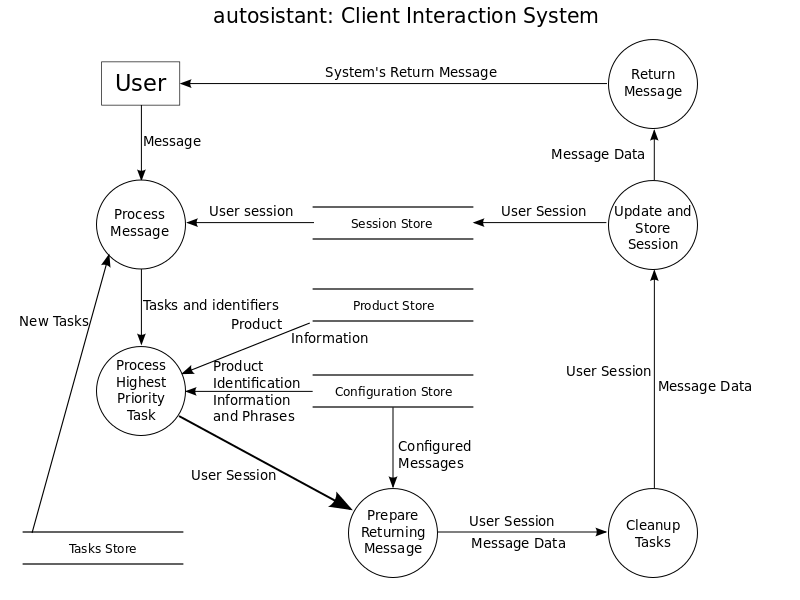
\includegraphics[scale=0.5]{project_dfd.png}
\subsection{DFD Summary}
The following is a brief summary of the data-flow diagram.

\begin{itemize}
\item \textbf{Session Store.}
The session information tied to a user, including her task queue, must be
stored from one turn to the next, since all messages are being sent
asynchronously, and the cost of storing the session variable is less than
sending the session variable on each AJAX call.
\item \textbf{Product Store.}
This is the companies own product data.  The system must be able to 
uniquely identify a product by its id field in the product table.  Other
information may be used from it as well.
\item \textbf{Configuration Store.}
This is the database that contains all configuration information for the
system.
\item \textbf{User.}
The user is the customer of the reseller.  The user must enter some message
to indicate what action she wishes to undertake.
\item \textbf{Process Message.}
After a user has entered a message for the system to analyze, the system
must find all the action words, interpret them as either immediately do-able
tasks (like ending the current session) or tasks that must be added to the task
list.  All other words are potential identifiers, and must be passed off
to the task in the task list that is the highest priority.  These priorities
are set within the Actions array in actions.rb.
\item \textbf{Process Highest Priority Task.}
As mentioned above, the system must then execute the task with the highest
priority.  As input, it takes all possible identifiers.
\item \textbf{Prepare Returning Message.}
The system must, at the end of processing the highest priority task, prepare
a return message to indicate to the user what action is required next, either
in the form of a question or a statement.  If the user input was erroneous,
then the system must return an appropriate message.
\item \textbf{Cleanup Tasks.}
If any tasks were completed, the system must remove it from the user's
task queue.
\item \textbf{Update and Store Session.}
Since the user session variable must be stored between messages to achieve
asynchronous communication, we must update the User's session information
appropriately, and store back in the Session Store.
\item \textbf{Return Message.}
Once all data handling has been done, all that is left is returning the message
to the User.
\end{itemize}

\end{document}

